\documentclass[10pt,landscape]{article}
\usepackage{multicol}
\usepackage{calc}
\usepackage{ifthen}
\usepackage[landscape]{geometry}
\usepackage{amsmath,amsthm,amsfonts,amssymb}
\usepackage{color,graphicx,overpic}
\usepackage{hyperref}


\pdfinfo{
  /Title (example.pdf)
  /Creator (TeX)
  /Producer (pdfTeX 1.40.0)
  /Author (Seamus)
  /Subject (Example)
  /Keywords (pdflatex, latex,pdftex,tex)}

% This sets page margins to .5 inch if using letter paper, and to 1cm
% if using A4 paper. (This probably isn't strictly necessary.)
% If using another size paper, use default 1cm margins.
\ifthenelse{\lengthtest { \paperwidth = 11in}}
    { \geometry{top=.5in,left=.5in,right=.5in,bottom=.5in} }
    {\ifthenelse{ \lengthtest{ \paperwidth = 297mm}}
        {\geometry{top=1cm,left=1cm,right=1cm,bottom=1cm} }
        {\geometry{top=1cm,left=1cm,right=1cm,bottom=1cm} }
    }

% Turn off header and footer
\pagestyle{empty}

% Redefine section commands to use less space
\makeatletter
\renewcommand{\section}{\@startsection{section}{1}{0mm}%
                                {-1ex plus -.5ex minus -.2ex}%
                                {0.5ex plus .2ex}%x
                                {\normalfont\large\bfseries}}
\renewcommand{\subsection}{\@startsection{subsection}{2}{0mm}%
                                {-1explus -.5ex minus -.2ex}%
                                {0.5ex plus .2ex}%
                                {\normalfont\normalsize\bfseries}}
\renewcommand{\subsubsection}{\@startsection{subsubsection}{3}{0mm}%
                                {-1ex plus -.5ex minus -.2ex}%
                                {1ex plus .2ex}%
                                {\normalfont\small\bfseries}}
\makeatother

% Define BibTeX command
\def\BibTeX{{\rm B\kern-.05em{\sc i\kern-.025em b}\kern-.08em
    T\kern-.1667em\lower.7ex\hbox{E}\kern-.125emX}}

% Don't print section numbers
\setcounter{secnumdepth}{0}


\setlength{\parindent}{0pt}
\setlength{\parskip}{0pt plus 0.5ex}

%My Environments
\newtheorem{example}[section]{Example}
% -----------------------------------------------------------------------

\begin{document}
\raggedright
\footnotesize
\begin{multicols}{3}


% multicol parameters
% These lengths are set only within the two main columns
%\setlength{\columnseprule}{0.25pt}
\setlength{\premulticols}{1pt}
\setlength{\postmulticols}{1pt}
\setlength{\multicolsep}{1pt}
\setlength{\columnsep}{2pt}

\begin{center}
     \Large{\underline{Computer Systems Cheat Sheet}} \\
\end{center}

\section{W1: Operating Systems}
\textbf{CPU cycle:} fetch, decode, execute, store.\\
\textbf{Registers:} hold variables and temporary results.\\
\textbf{Special registers:} program counter (PC), stack pointer (SP), program status word (PSW).\\
\textbf{User mode:} restricted access to memory and instructions.\\
\textbf{Kernel mode:} full access to the above.\\
\textbf{Memory stack:}\\
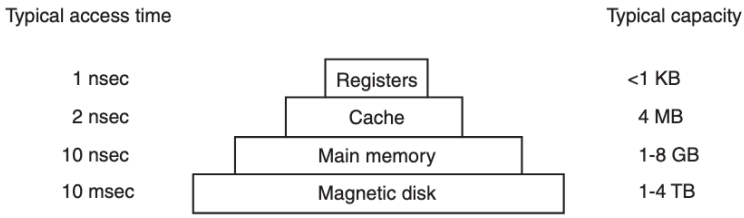
\includegraphics[width=\linewidth]{figs/memory-stack.png}

\subsection{System calls}
\begin{enumerate}
    \item Put system call number in register of OS.
    \item Execute trap instruction (switch to kernel mode).
    \item OS executes system call from fixed address in kernel memory.
    \item The kernel code that starts following the trap instruction is called the \textbf{trap handler}. Trap handler examines the system call number and dispatches the correct system-call handle.
    \item System call handler runs.
    \item Return to user mode.
\end{enumerate}

\section{W2: Processes, Threads}
\textbf{Why processes?} Simultaneous execution of multiple programs on single CPU.\\
\textbf{Why threads?} Simultaneous execution of multiple parts of a program on single CPU. Threads share global variables and heap memory.\\

\subsection{Interprocess communication}
\textit{Process/Thread Synchronization} Race conditions occur when multiple processes/threads access shared data and try to change it at the same time.\\
\textbf{Critical region:} code segment where shared data is accessed.\\
\textbf{Mutual exclusion:} only one process/thread can be in critical region at a time.\\
\begin{enumerate}
    \item No two processes/threads may be simultaneously inside their critical regions.
    \item No assumptions may be made about speeds or the number of CPUs.
    \item No process/thread running outside its critical region may block other processes/threads.
    \item No process/thread should have to wait forever to enter its critical region.
\end{enumerate}

\subsubsection{Possible approaches to mutual exclusion}
\textbf{Busy waiting:} process/thread stays in loop in kernel mode until it can enter critical region. Pros: simple, no context switch. Cons: wastes CPU time, starvation (Priority Inversion Problem).\\
\begin{enumerate}
    \item \textbf{Lock variables:} each process/thread has a lock variable. Process/thread can enter critical region only if its lock variable is 0.\\
    \item \textbf{Strict alternation:} processes/threads take turns entering critical region.\\
    \item \textbf{Peterson's solution:} two processes/threads, two lock variables.\\
    \item \textbf{Test-and-set (TSL):} atomic instruction that sets lock variable to 1 and returns old value.\\
\end{enumerate}

\subsubsection{Deadlocks}
Four conditions for deadlock:
\begin{enumerate}
    \item \textbf{Mutual exclusion:} only one process/thread can use a resource at a time.
    \item \textbf{Hold and wait:} processes/threads hold resources while waiting for others.
    \item \textbf{No preemption:} resources can be released only voluntarily by process/thread holding it.
    \item \textbf{Circular wait:} two or more processes/threads form a circular chain where each process/thread waits for a resource held by next process/thread in chain.
\end{enumerate}
\section{W3: Scheduling, Memory Management}
\textbf{Preemption:} Preemptive scheduling is when the scheduler decides to switch to another process/thread. Clock interrupts used upon a quantum. Non-preemptive scheduling is when the process/thread itself decides to give up the CPU or is blocked.\\
\textbf{Context switch:} Switching from one process/thread to another is expensive.\\

\subsection{Non-preemptive scheduling}
\textbf{First-come, first-served (FCFS):} Simple, but long average waiting time.\\
\textbf{Shortest job first (SJF):} Shortest average waiting time, but long waiting time for long processes/threads. Average turnaround time is minimized.\\

\subsection{Preemptive scheduling}
\textbf{Round-robin (RR):} Each process/thread gets a quantum.\\
\textbf{Shortest remaining time first (SRTF):} Shortest average waiting time, but long waiting time for long processes/threads. Average turnaround time is minimized.\\
\textbf{Priority scheduling:} Each process/thread has a priority. May lead to starvation.\\

\subsection{Memory management}
\textbf{Why Memory Management?} Support multiprogramming. Secure isolation between processes/threads and OS memory. Enables virtual memory which allows processes/threads to use more memory than is physically available.\\
\textbf{No memory abstraction:} Use swap space on disk. Multiplex physical memory.\\

\subsubsection{Memory abstraction}
\textbf{Logical address space:} set of addresses that a process/thread can use which are mapped to physical addresses.\\
\textbf{Base and limit registers:} base register holds start address of process/thread, limit register holds size of process/thread.\\
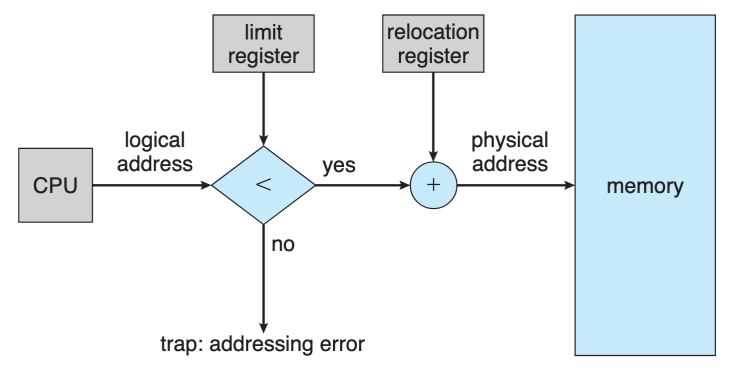
\includegraphics[width=\linewidth]{figs/base-and-limit-registers.png}
\textbf{Memory management unit (MMU):} hardware device that maps logical addresses to physical addresses.\\
\textbf{Manage free memory:} using bitmap or linked list.\\
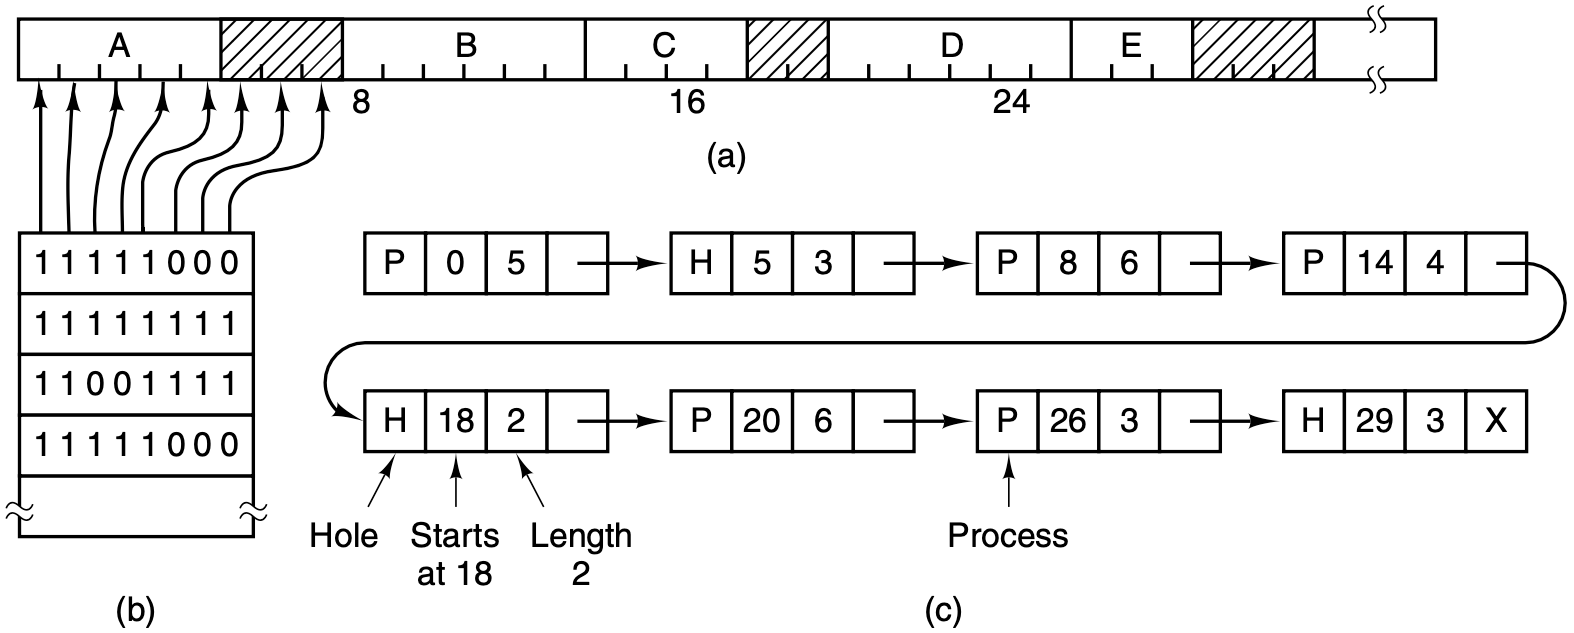
\includegraphics[width=\linewidth]{figs/memory-management.png}

\subsubsection{Virtual memory}
\textbf{Why virtual memory?} Processes/threads can use more memory than is physically available.\\
\textbf{Page table:} maps virtual pages to physical pages.\\
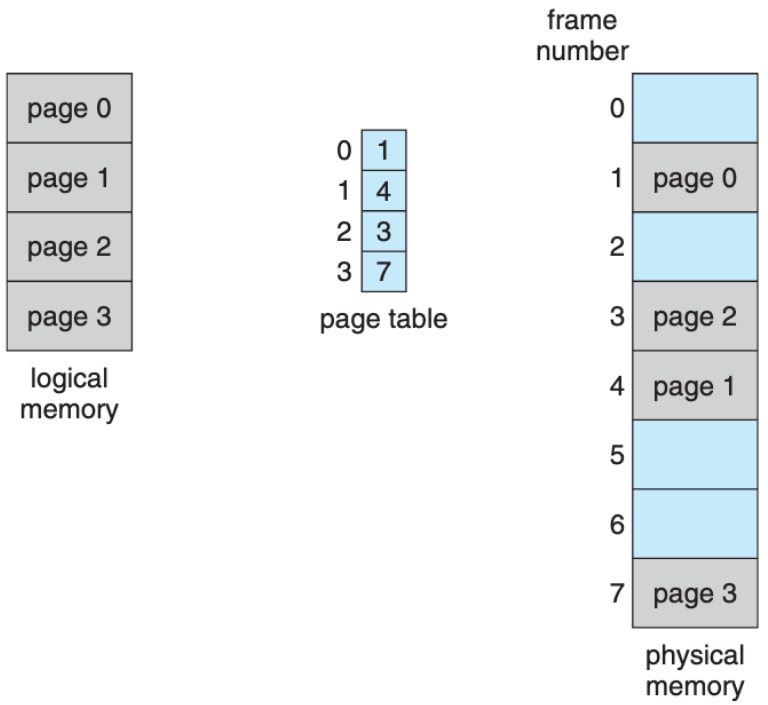
\includegraphics[width=0.4\linewidth]{figs/paging-model.png}
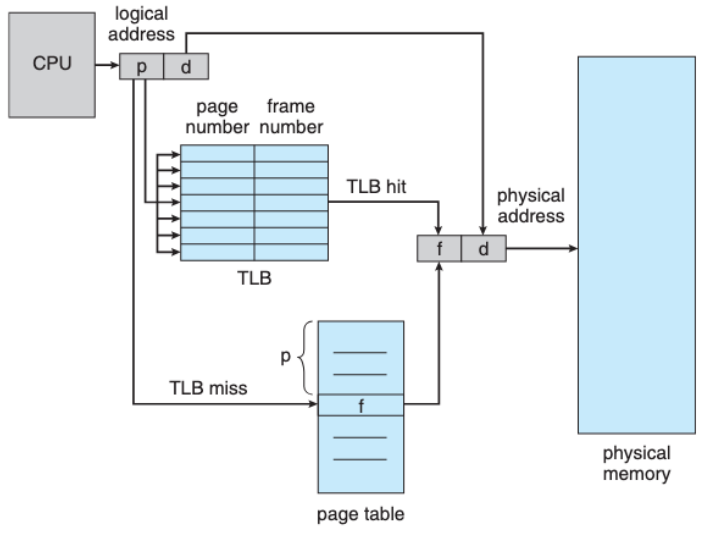
\includegraphics[width=0.45\linewidth]{figs/mmu-with-tlb.png}\\
\textbf{Translation Lookaside Buffer (TLB):} cache for page table, faster than main memory, speeds up address translation.\\
\textbf{Page replacement algorithms for TLB:} \textit{NRU} (Not Recently Used, R and M bit, 4 classes between referenced and modified).\\


% % You can even have references
% \rule{0.3\linewidth}{0.25pt}
% \scriptsize
% \bibliographystyle{abstract}
% \bibliography{refFile}
\end{multicols}
\end{document}